\section{Current Solutions}
\label{section:current-solutions}
The Unified Cross Domain Management Office (UCDMO) supports efforts to develop specific solutions to cross-domain information sharing.  Solution architectures have been presented over the past few years to handle this kind of information management.  The National Security Agency set the standard in this area initially.  In 2009, at a conference sponsored by the UCDMO, Booz Allen Hamilton (BAH) and Raytheon presented alternative notional architectures contrasting with current NSA-influenced approaches ~\cite{proposal:nsa-arch,proposal:gig-arch,proposal:bah-arch,proposal:raytheon-arch}.

The current standard architectural model in place and governed by the UCDMO to deal with these kinds of issues are guard-centric cross domain architectures.  As we will show, the thinking behind these system architectures has remained relatively static over the past 20 years.  New thinking with regard to future internet architectures and usage management provide more powerful approaches to securing information as it flows through dynamic systems.

Current and near-future proposed solutions endorsed by the UCDMO include system architectures assembled by the NSA, Raytheon, and Booz $\mid$  Allen $\mid$  Hamilton (BAH).   The NSA has been active in this area for decades as a logical extension of their role in signals intelligence collection and processing.  Raytheon and BAH have been engaged over the past few years to provide an alternative voice and design approach to these kinds of systems, an effort met with limited success.


\begin{figure}[!t]
\centering
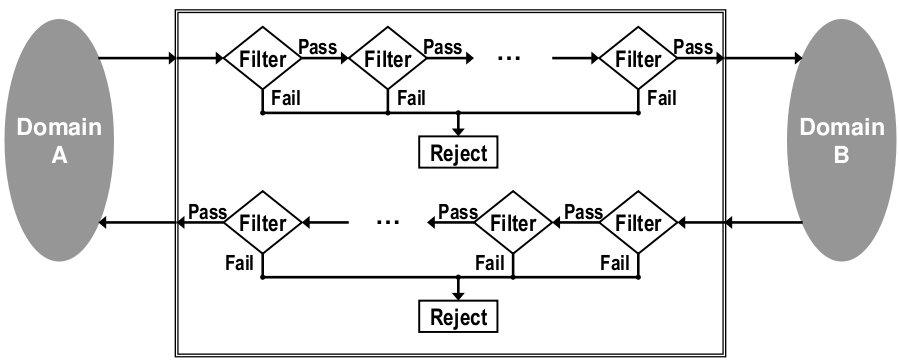
\includegraphics[width=5in]{nsa-legacy-arch}
\caption{NSA Legacy Notional Architecture Model}
\label{fig:model:conceptual-model}
\end{figure}

These cross-domain solutions are intended to enable sensitive information to easily flow both from a higher sensitivity domain to a lower sensitivity domain, and from lower to higher as well.  They generally act over both primary data (say, a document) and metadata over that primary data.

\subsection{NSA, Filtered}
The NSA conducted initial work in this area.  Their standard-setting efforts culminated in a reasonable conceptual system architecture, using groups of filters dedicated to specific delineated tasks to process sensitive information ~\cite{proposal:nsa-arch}. In the scenario portrayed in Figure ~\ref{fig:model:conceptual-model}, \textit{Domain A} could very well be a private cloud managed by the U.S. Air Force, while \textit{Domain B} is a public operational network of some kind shared by coalition partners in a joint operation.

A system user attempts to send a \textit{data package} consisting of a primary document and associated metadata from \textit{Domain A} to \textit{Domain B}.  At some point, that submission reaches a \textit{guard}, which contains at least one \textit{filter chain}.  Each filter chain then contains at least one \textit{filter}.  Individual filters can execute arbitrary actions over a submitted data package and have access to any number of external resources as required.  At any point, a filter can examine the data package and reject it, at which point it will frequently wait for human review.  If a filter does not reject a data package, it passes that package onto the next filter or submits it for delivery to Domain B.

\subsection{NSA, Services}
In recent years, the NSA has extended the legacy system architecture for cross-domain information sharing to exploit service-oriented computing styles ~\cite{proposal:nsa-arch}.  Visualized in Figure ~\ref{fig:model:conceptual-model-services}, this model incorporates more modern conceptual elements and componentry.

Figure ~\ref{fig:model:conceptual-model-services} shows on the left the \textit{Global Information Grid}, or \textit{GIG}.  On the right, the \textit{Distributed Service-oriented Cross Domain Solution}, or \textit{DSCDS}.  The GIG is not a truly open system --- rather, it is a loosely coupled collection of computational services handing data at a variety of levels of sensitivity, federated to provide stakeholders timely access to relevant information ~\cite{proposal:gig-arch}.  The DSCDS is essentially the embodiment of the NSA's cross-domain vision applied to service oriented computing.  This model fuses various technology choices with previous cross-domain thinking.

\begin{figure}[!t]
\centering
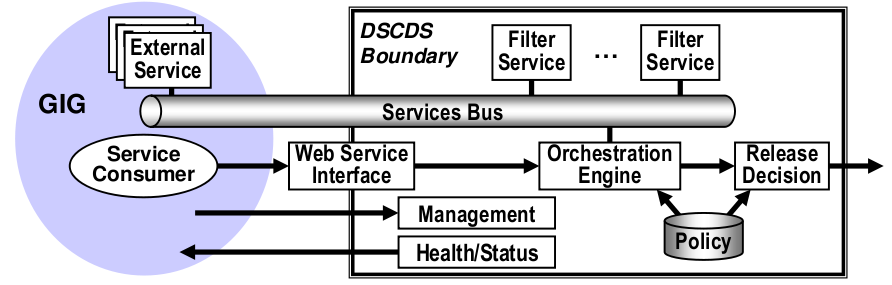
\includegraphics[width=5in]{nsa-arch}
\caption{NSA Service-Oriented Model}
\label{fig:model:conceptual-model-services}
\end{figure}

Indicative of this more modern system design thinking, a variety of services and service consumers are attached to a common service bus within the GIG.  Within the DSCDS, groups of filters are implemented as services inspecting transferred data when moved over the bus.  Finally, all of this interaction is managed by a management interface and controlled by an orchestration engine accessing a centralized group of policies.

Note that here a common policy repository for various types of security metadata over primary data elements has begun to be accessed.

\subsection{Raytheon}
In the past few years, Raytheon has offered a new model for cross domain use influenced by the NSA service-oriented model ~\cite{proposal:raytheon-arch}.  The model in Figure ~\ref{fig:model:conceptual-model-ray} is more grounded in the actual technical environment this kind of solution would be embedded within.  The Non-secure Internet Protocol Router Network (NIPRNet) is one domain, and the Secret Internet Protocol Router Network (SIPRNet) is the other.  Here, NIPRNet is the lower security domain (lowside), and SIPRNet the higher security domain (highside).  This particular view shows the motion of data from the high side (SIPRNet) to the low side (NIPRNet).

\begin{figure}[!t]
\centering
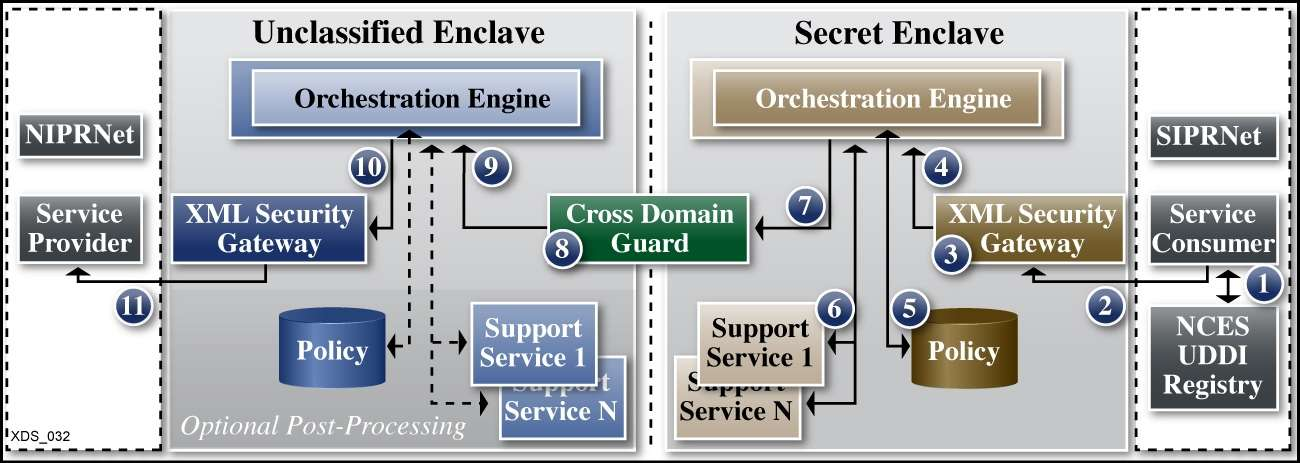
\includegraphics[width=5in]{raytheon-arch}
\caption{Ratheon Model}
\label{fig:model:conceptual-model-ray}
\end{figure}

Here, a data request is submitted from SIPRNet first to the \textit{XML Security Gateway} which calls into the \textit{Orchestration Engine} for policy validation.  The Orchestration Engine then coordinates calls into a \textit{Policy Repository} as well as to a collection of external \textit{Support Services}.  Once rectified against these elements, the request is passed into the \textit{Cross Domain Guard} which routes the request into the \textit{Unclassified Enclave} in NIPRNet.  Here, the request is passed directly through the lowside \textit{XML Security Gateway}, without rectification, onto the \textit{Service Provider}.  The response from the Service Provider is then passed back to the requester via the inverse path.

This model also begins to use a centralized policy repository, just as the NSA Service Model does.  It also uses a single cross domain guard to transfer information from both the highside to the lowside, and vice-versa.

\subsection{Booz $\mid$ Allen $\mid$ Hamilton}
BAH submitted a competing model, also in 2009 ~\cite{proposal:bah-arch}.  In fact, both Raytheon and BAH presented their models under competitive contract to the UCDMO at the same conference, so the domain application is not coincidental.  Figure ~\ref{fig:model:conceptual-model-bah} embodies BAH's thinking with respect to cross domain information management.  It showcases a \textit{Domain A} as a high security domain, and \textit{Domain B} as a low security domain.  Here, dataflow again exists from the highside to the lowside through the cross domain management system.

\begin{figure}[!t]
\centering
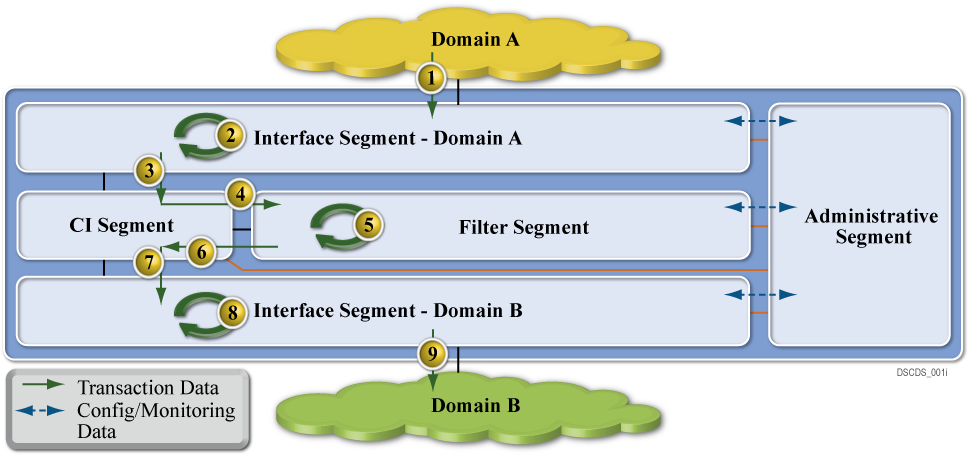
\includegraphics[width=5in]{bah-arch}
\caption{Booz $\mid$ Allen $\mid$ Hamilton Model}
\label{fig:model:conceptual-model-bah}
\end{figure}

While not as detailed as the Raytheon proposal, this does have similar elements.  Here, the data first travels from Domain A into the \textit{Interface Segment for Domain A}, similar to the secret enclave used in the Raytheon model.  From there, it moves into the \textit{CI Segment}, which in turn submits the transferring data into the \textit{Filter Segment}.  From there, the package is moved into the \textit{Interface Segment for Domain B}, and then onto \textit{Domain B}.  The \textit{Administrative Segment} provides management and oversight of the system as a whole.  Note the absence of specific policy-centric elements.  This system is reliant on specific policy-agnostic content filters as well.